% Cascaded Bengali-to-English Speech Translation Pipeline: procedure briefing
% Compile with XeLaTeX (needed for Bengali script)
\documentclass[11pt,a4paper]{article}

% Packages, fonts, boxes and macros for the speech translation pipeline report
\usepackage[margin=2.5cm]{geometry}
\usepackage{fontspec}
\setmainfont{Latin Modern Roman}
\newfontfamily\bn{Nirmala UI}[Script=Bengali,Scale=0.80]
\usepackage{booktabs,tabularx,array}
\usepackage{xcolor}
\usepackage{enumitem}
\usepackage{fontawesome5}
\usepackage{tikz}
\usetikzlibrary{arrows.meta,positioning,calc}
\usepackage[backend=biber,style=numeric,sorting=none,urldate=long]{biblatex}
\addbibresource{references.bib}
% Bibliography URLs: allow breaks at any character and set entries ragged-right,
% so that long URLs are not stretched with visible gaps
\setcounter{biburlnumpenalty}{100}
\setcounter{biburlucpenalty}{100}
\setcounter{biburllcpenalty}{100}
\renewcommand*{\bibfont}{\raggedright}
\usepackage[colorlinks=true,linkcolor=blue!50!black,citecolor=blue!50!black,urlcolor=blue!50!black]{hyperref}

\usepackage[most]{tcolorbox}
% Worked-example box: breakable, but never between a paragraph and the diagram that follows it
% (no page break before a centred diagram and no split inside a paragraph), so a box splits
% only after a diagram.
\newtcolorbox{example}[1][]{breakable, enhanced, colback=green!4, colframe=green!40!black,
  before upper={\csname @beginparpenalty\endcsname=10000 \interlinepenalty=10000 \clubpenalty=10000 \widowpenalty=10000 },
  boxrule=0.6pt, arc=3pt, left=6pt, right=6pt, top=4pt, bottom=4pt, fontupper=\small,
  title={From example#1}, fonttitle=\bfseries\small, coltitle=white,
  before skip=10pt, after skip=10pt}

\newcommand{\stagecontent}[5][8.9cm]{\parbox[c]{1.4cm}{\centering\color{#2}\fontsize{24}{24}\selectfont #3}\hspace{1mm}\parbox[c]{#1}{\centering{\bfseries #4}\\[2pt]\small #5}}
\newcommand{\model}[1]{\texttt{\small #1}}
\newcommand{\source}[1]{{\footnotesize\color{black!60}#1}}
% Worked example data. All values are taken from the pipeline run on the example clip.

\def\clipduration{6.48}  % length of the original clip (s)

% One entry per word, in spoken order.
%   Bengali / romanized / romanization note (ok or lossy)
\def\romanization{%
  গ্রেগরির/gregarir/lossy,
  কাছ/kaachh/ok,
  থেকে/theke/ok,
  এখনও/ekhanao/ok,
  উত্তর/uttar/ok,
  পেলাম/pelaam/ok,
  না/naa/ok,
  সে/se/ok,
  কি/ki/ok,
  তাহলে/taahale/ok,
  ইংল্যাণ্ডে/inglyaanndde/lossy,
  নেই/nei/ok}

% One entry per word, in spoken order.
%   romanized / start (s) / end (s) / silence flag (none, gap or short) /
%   loudness z-score / emphasis (none, loud or soft) / length ratio / dragged (no or yes)
\def\words{%
  gregarir/0.62/1.10/gap/0.96/loud/1.42/yes,
  kaachh/1.14/1.38/none/-0.02/none/0.95/no,
  theke/1.40/1.62/none/0.24/none/1.04/no,
  ekhanao/1.80/2.09/none/-0.11/none/0.95/no,
  uttar/2.17/2.39/none/-0.67/none/1.04/no,
  pelaam/2.43/2.71/none/-0.26/none/1.11/no,
  naa/2.79/2.89/none/-2.87/soft/0.79/no,
  se/3.87/3.97/gap/0.52/none/1.18/yes,
  ki/4.05/4.13/none/0.72/none/0.96/no,
  taahale/4.17/4.45/none/1.20/loud/0.95/no,
  inglyaanndde/4.53/4.95/none/0.10/none/0.83/no,
  nei/5.07/5.32/none/0.19/none/1.90/yes}

% Pauses that were marked, placed at the middle of their silence.
%   position (s) / type (short or long) / length of the silence (s)
\def\pauses{%
  3.38/long/0.98}

% Pause thresholds (s).
\def\shortthreshold{0.20}  % a short pause is at least this long
\def\longthreshold{0.50}   % a long pause is at least this long

% Silences between consecutive words (s), compared with the pause thresholds.
\def\innergaps{0.04, 0.02, 0.18, 0.08, 0.04, 0.08, 0.98, 0.08, 0.04, 0.08, 0.12}
% Silence before the first word and after the last word (s).
\def\edgegaps{0.62, 1.16}
  % worked example data
\setlength{\parskip}{4pt}
\setlength{\emergencystretch}{3em}


\title{\textbf{Cascaded Bengali-to-English Speech Translation Pipeline}}
\author{Sayan Gupta}
\date{\today}

\begin{document}
\maketitle

\begin{abstract}
\noindent This report describes a cascaded procedure for translating Bengali speech into English speech while keeping the original speaker's voice and phrasing. A Bengali clip is transcribed, each word is located in time by forced alignment, the word timings are used to mark where the speaker pauses, and the timings and signal energy are used to measure which words are louder or elongated. The marked Bengali text is translated into English, and the translation is spoken by a zero-shot voice-cloning speech synthesizer that uses the original clip as its voice reference. The report describes each stage and the reasoning behind it, and it lists the open issues that have been identified so far.
\end{abstract}


\tableofcontents
\newpage

\begin{figure}[p]
\centering
% The five stages of the pipeline, with romanization as a side branch.
\begin{tikzpicture}[
  stage/.style={draw=blue!55!black, rounded corners=4pt, fill=blue!7, line width=0.8pt,
                minimum width=10.9cm, minimum height=2.0cm, inner sep=6pt,
                execute at begin node={\hyphenpenalty 10000\relax}},
  rule/.style={stage, draw=orange!70!black, fill=orange!10},
  io/.style={draw=black!60, rounded corners=10pt, fill=black!5, line width=0.8pt,
             text width=5.2cm, minimum height=1.0cm, align=center, font=\small},
  data/.style={font=\footnotesize\itshape, text=black!70, anchor=west, align=left, text width=6.6cm},
  arr/.style={-{Stealth[length=3mm]}, line width=1pt},
  title/.style={font=\bfseries\large}
]
% ---- nodes ----
\node[io] (in) at (0,0) {\faIcon{microphone}\ \textbf{Input:} Bengali speech clip\\ \footnotesize (the original recording)};

\node[stage] (asr) at (0,-2.4) {\stagecontent{blue!55!black}{\faIcon{file-alt}}{1. Transcription}
  {Converts the Bengali speech into Bengali text written in native script.}};

% Romanization forms a side branch; the transcript itself goes straight to Stage 3.
\node[rule, minimum width=6.5cm] (rom) at (2.2,-5.2) {\stagecontent[4.6cm]{orange!70!black}{\faIcon{font}}{2. Romanization}
  {Rewrites each word in Latin letters for the aligner.}};

\node[stage] (pro) at (0,-8.0) {\stagecontent{blue!55!black}{\faIcon{wave-square}}{3. Alignment and prosody marking}
  {Finds when each word starts and ends, then inserts \texttt{,} for short pauses and \texttt{|} for
  long pauses; also measures loudness and elongated words.}};

\node[stage] (tr) at (0,-10.8) {\stagecontent{blue!55!black}{\faIcon{language}}{4. Translation}
  {Translates the pause-marked Bengali text into English.}};

\node[stage] (tts) at (0,-13.6) {\stagecontent{blue!55!black}{\faIcon{volume-up}}{5. Voice-cloned speech synthesis}
  {Speaks the English text in the original speaker's voice, copied zero-shot from the input clip.}};

\node[io] (out) at (0,-16.1) {\faIcon{headphones}\ \textbf{Output:} English speech\\ \footnotesize in the original speaker's voice};

% ---- main flow with data labels ----
\draw[arr] (in)  -- node[data, xshift=2mm]{audio} (asr);
\draw[arr] (asr.south -| rom) -- node[data, xshift=2mm, text width=3cm]{Bengali words} (rom);
\draw[arr] (rom) -- node[data, xshift=2mm, text width=3cm]{romanized words} (rom.south |- pro.north);
\draw[arr] (asr.south -| -3.8,0) -- node[data, xshift=2mm, text width=2.4cm]{Bengali text, no punctuation} (pro.north -| -3.8,0);
\draw[arr] (pro) -- node[data, xshift=2mm]{Bengali sentence with pause markers} (tr);
\draw[arr] (tr)  -- node[data, xshift=2mm]{English translation} (tts);
\draw[arr] (tts) -- node[data, xshift=2mm]{synthesized audio} (out);

% the aligner also needs the audio
\draw[arr] (in.east) -- (6.3,0) |- (pro.east);
\node[font=\footnotesize\itshape, text=black!70, rotate=90, anchor=south] at (6.3,-4.0) {audio};

% ---- side inputs ----
\draw[arr, dashed, black!55] (in.west) -- (-6.6,0) |- ([yshift=4mm]tts.west);
\node[font=\footnotesize\itshape, text=black!65, rotate=90, anchor=south] at (-6.6,-6.8)
  {original clip reused as the voice reference};

\draw[arr, dashed, black!55] ([yshift=-4mm]pro.west) -- (-5.8,-8.4) |- ([yshift=-4mm]tts.west);
\node[font=\footnotesize\itshape, text=black!65, rotate=90, anchor=south] at (-5.8,-11.0)
  {marked Bengali as transcript};
\end{tikzpicture}


\vspace{4mm}
{\small \tikz\node[draw=blue!55!black, fill=blue!7, rounded corners=2pt, minimum width=6mm, minimum height=3.5mm]{}; \ stage using a pretrained model\qquad \tikz\node[draw=orange!70!black, fill=orange!10, rounded corners=2pt, minimum width=6mm, minimum height=3.5mm]{}; \ rule-based stage\qquad \tikz\draw[-{Stealth}, dashed, black!55, line width=1pt](0,0)--(6mm,0); \ side input to speech synthesis}

\caption{The five stages of the speech translation pipeline, from top to bottom.}
\label{fig:pipeline}
\end{figure}
\clearpage

%=====================================================================
\section{Overview}
%=====================================================================

The central idea is that a plain transcript loses the speaker's rhythm. Automatic transcripts contain no punctuation, so the translator cannot tell where one thought ends and the next begins, and the speech synthesizer has no cue for where to pause. Recovering the pauses from the audio and writing them back into the text is intended to supply this information to both downstream models.

\begin{table}[h]
\centering\small
\renewcommand{\arraystretch}{1.25}
\begin{tabularx}{\linewidth}{@{}>{\raggedright\arraybackslash}p{2.2cm}
  >{\raggedright\arraybackslash}p{4.4cm} >{\raggedright\arraybackslash}X
  >{\raggedright\arraybackslash}p{4.1cm}@{}}
\toprule
\textbf{Stage} & \textbf{Model} & \textbf{Type} & \textbf{Input $\rightarrow$ output} \\
\midrule
Transcription & \model{indic-transcribe-core}\newline\source{bodhan-ai}~\cite{bodhan-transcribe}
  & Speech recognition model for Indic languages
  & Bengali speech $\rightarrow$ Bengali text \\
Romanization & \model{uroman}\newline\source{isi-nlp}~\cite{hermjakob2018uroman}
  & Rule-based universal romanizer
  & Bengali text $\rightarrow$ Latin-script text \\
Alignment and prosody marking & \model{MMS\_FA}\newline\source{torchaudio}~\cite{pratap2024mms,yang2022torchaudio}
  & Multilingual acoustic model trained with CTC~\cite{graves2006ctc} on romanized text, followed by rule-based signal analysis
  & Speech, romanized words and Bengali text $\rightarrow$ pause-marked Bengali text \\
Translation & \model{indic-translate}\newline\source{bodhan-ai}~\cite{bodhan-translate}
  & Instruction-following multilingual language model
  & Bengali text $\rightarrow$ English text \\
Speech synthesis & \model{higgs-audio-v3-\allowbreak tts-4b-transformers}\newline\source{multimodalart}~\cite{multimodalart-higgs}
  & Zero-shot voice-cloning speech synthesis model
  & English text and reference speech $\rightarrow$ English speech \\
\bottomrule
\end{tabularx}
\caption{Models used in the pipeline.}
\label{tab:models}
\end{table}

%=====================================================================
\section{Transcription}
%=====================================================================

The input is a Bengali speech clip. It is transcribed by the transcription model (Table~\ref{tab:models}), with the language set to Bengali. The output is a single string of Bengali text in native script, and \textbf{it contains no punctuation}.

\begin{example}[: transcription]
The diagram shows the audio of the clip, which lasts \textbf{6.48\,s}, and the text that the transcription model produced from it.

\begin{center}
% Worked example, Stage 1: the audio of the clip and the text transcribed from it.
% The x axis is in seconds (1 s = 2.1 cm).
\begin{tikzpicture}[x=2.1cm]
  \pgfmathtruncatemacro\lastsecond{\clipduration}
  \pgfmathsetmacro\middle{\clipduration/2}

  % Audio envelope of the clip
  \begin{scope}[yscale=0.6]
    \fill[black!25] plot file {figures/data/original-envelope.dat} -- cycle;
  \end{scope}
  \node[font=\footnotesize\itshape, text=black!60, anchor=south west] at (0,0.75)
    {audio envelope of the clip};

  % Time axis
  \draw[black!60] (0,-0.7) -- (\clipduration,-0.7);
  \foreach \t in {0,...,\lastsecond}
    \draw[black!60] (\t,-0.7) -- ++(0,-0.08)
      node[below, font=\scriptsize] {\t\,s};

  % Transcription
  \draw[-{Stealth[length=2.5mm]}, line width=1pt] (\middle,-1.15) -- (\middle,-1.95)
    node[midway, right, font=\footnotesize\itshape, text=black!65] {transcription model};
  \node[draw=blue!55!black, fill=blue!5, rounded corners=3pt, text width=13.2cm,
        align=center, inner sep=6pt, anchor=north] at (\middle,-2.05)
    {\bn গ্রেগরির কাছ থেকে এখনও উত্তর পেলাম না সে কি তাহলে ইংল্যাণ্ডে নেই};
\end{tikzpicture}

\end{center}

\end{example}

%=====================================================================
\section{Romanization}
%=====================================================================

The forced aligner used in the next stage was trained on romanized text, and it only recognizes the Latin letters a-z and the apostrophe. Each Bengali word is therefore converted to a Latin spelling by the romanizer (Table~\ref{tab:models}), and any remaining characters outside that set are removed. Words keep a link back to their original Bengali form, so that later stages can work with the native script again.

\begin{example}[: romanization]
The diagram shows each Bengali word above its romanized form. The two words outlined in red are English names written in Bengali script. \textbf{Neither romanization matches the English pronunciation}, and the doubled letters in \texttt{inglyaanndde} make the word look longer than it sounds.

\begin{center}
% Worked example, Stage 2: each Bengali word above its romanized form.
% Words are laid out in a grid of 6 columns; lossy romanizations are outlined in red.
\begin{tikzpicture}[
    cell/.style={rounded corners=2pt, minimum width=2.3cm, minimum height=1.35cm},
    ok/.style={draw=blue!55!black, text=blue!55!black},
    lossy/.style={draw=red!70!black, fill=red!6, text=red!70!black},
  ]
  \foreach [count=\i from 0] \bengali/\romanized/\note in \romanization {
    \pgfmathtruncatemacro\col{mod(\i,6)}
    \pgfmathtruncatemacro\row{div(\i,6)}
    \begin{scope}[shift={({\col*2.45},{-\row*1.55})}]
      \node[cell, \note] at (0,-0.2) {};
      \node at (0,0.08) {\bn \bengali};
      \draw[-{Stealth[length=1.5mm]}, \note] (0,-0.12) -- (0,-0.36);
      \node[font=\scriptsize\ttfamily, \note, draw=none, fill=none] at (0,-0.55) {\romanized};
    \end{scope}
  }
\end{tikzpicture}

\end{center}
\end{example}

%=====================================================================
\section{Alignment and Prosody Marking}
%=====================================================================

This stage recovers the speaker's delivery from the audio and writes it back into the Bengali text as inline markers. It first locates each word in time by forced alignment, and it then analyzes the word timings and the raw waveform with fixed rules to mark pauses and to measure loudness and elongation. Only the alignment step uses a model.

\subsection{Forced alignment}
Forced alignment determines where each known word occurs in the audio. Because the aligner (Table~\ref{tab:models}) was trained on romanized text in many languages, it can be used for Bengali without a language-specific aligner.

The audio is mixed to mono and resampled to \textbf{16\,kHz}. The model produces character probabilities for every short frame of audio, and the aligner finds the most likely path of the known characters through those frames. This gives each word a start time and an end time, which the following steps use.

\subsection{Pauses}
The silence before each word is measured and compared with two fixed thresholds:
\begin{itemize}[nosep]
  \item A \textbf{short pause}, marked with a comma (\texttt{,}), is any gap of at least \textbf{0.20\,s} and shorter than 0.50\,s.
  \item A \textbf{long pause}, marked with a bar (\texttt{|}), is any gap of at least \textbf{0.50\,s}.
\end{itemize}
The silence before the first word and the silence after the last word are not marked.

\subsection{Loudness}
The waveform is split into \textbf{25\,ms} frames, and the energy of each frame is measured in decibels. A word's loudness is the average of its loudest frames, so that brief dips do not pull it down. Each word is then compared with the rest of the clip. Words well above the clip's typical loudness are marked \emph{loud}, and words well below it are marked \emph{soft}.

\subsection{Elongated words}
Speakers often elongate a word for effect. Since a longer word naturally takes longer to say, its duration is divided by its romanized length to obtain a time per character. Each word is then compared with the clip's median time per character, and a word that is unusually slow for its length is marked \emph{dragged}.

\subsection{The marked sentence}
The Bengali words are rebuilt into a sentence, with each pause marker placed before the word that follows the pause. \textbf{In the current procedure only the pause markers reach translation and synthesis.} Loudness and elongation are still measured and reviewed.

\begin{example}[: alignment and prosody marking]
The first diagram shows the result of the stage on the time axis of the clip. Each word has its own column, which follows a dotted guide from its aligned position down to its loudness relative to the clip average and its duration relative to the duration expected for its romanized length.

\begin{center}
% Worked example, alignment and prosody marking: one panel on the time axis of the clip
% (1 s = 1.45 cm), with one column per word. Each column holds the word's aligned block (below
% the audio envelope), its name, its loudness bar and its length bar, joined by a faint vertical
% guide. Names are vertical (90 degrees) and small, hanging below their blocks. Row titles are on
% the left and the legend is on the right. Row positions (y, cm):
%   audio envelope 0, word blocks -0.55, names from -0.80 down,
%   loudness baseline -3.00, length baseline -5.70, time axis -5.85.
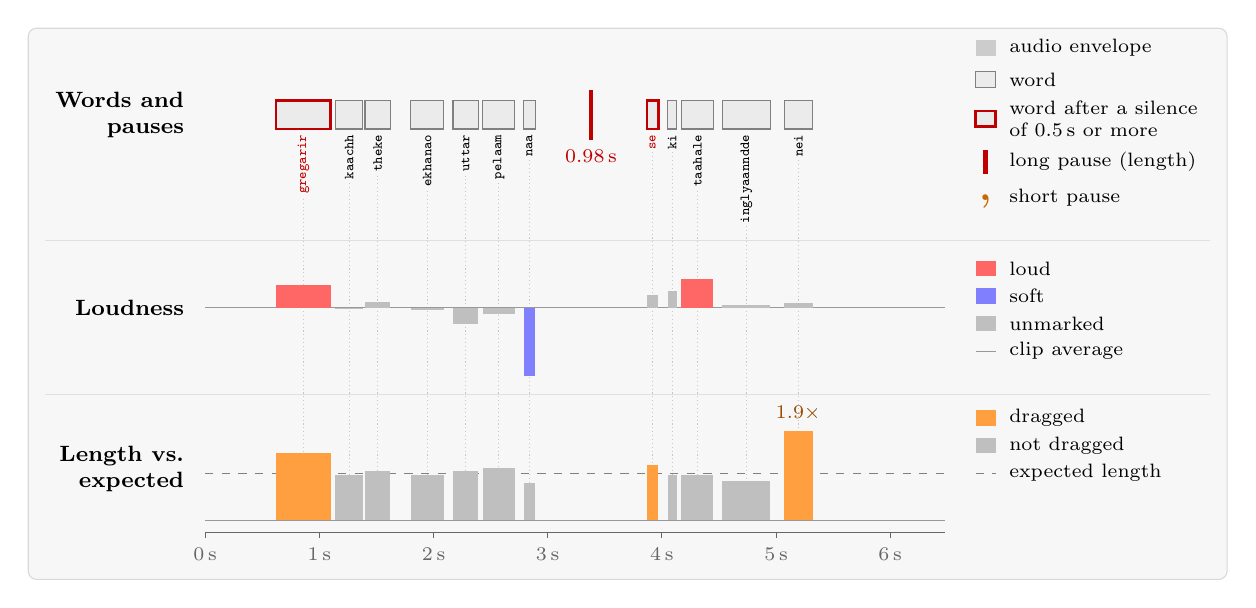
\begin{tikzpicture}[x=1.45cm,
    emph none/.style={fill=black!25},
    emph loud/.style={fill=red!60},
    emph soft/.style={fill=blue!50},
    drag no/.style={fill=black!25},
    drag yes/.style={fill=orange!75},
    flag none/.style={draw=black!50},
    flag gap/.style={draw=red!75!black, line width=1pt},
    flag short/.style={flag gap},
    label none/.style={},
    label gap/.style={text=red!75!black},
    label short/.style={label gap},
    panel/.style={fill=black!3, draw=black!15, rounded corners=3pt},
    row title/.style={font=\footnotesize\bfseries, align=right, anchor=east},
    legend/.style={font=\scriptsize, anchor=west},
    guide/.style={black!22, densely dotted},
  ]
  \pgfmathtruncatemacro\lastsecond{\clipduration}
  \def\legendx{6.75}   % where the legend starts (s)
  \def\wordy{-0.55}    % centre of the word blocks
  \def\loudy{-3.00}    % loudness baseline (clip average)
  \def\lengthy{-5.70}  % length baseline (zero length)

  % One panel for all rows
  \fill[panel] (-1.55,0.55) rectangle (8.95,-6.45);

  % Row titles
  \node[row title] at (-0.1,-0.55)   {Words and\\pauses};
  \node[row title] at (-0.1,\loudy)  {Loudness};
  \node[row title] at (-0.1,-5.05)   {Length vs.\\expected};

  % Faint row separators
  \draw[black!12] (-1.4,-2.15) -- (8.8,-2.15);
  \draw[black!12] (-1.4,-4.10) -- (8.8,-4.10);

  % Guides: one per word, from its block down through the loudness and length rows
  \foreach \word/\tstart/\tend/\flag/\loudz/\emphasis/\ratio/\dragged in \words
    \draw[guide] ({(\tstart+\tend)/2},{\wordy-0.18}) -- ({(\tstart+\tend)/2},\lengthy);

  % Reference lines
  \draw[black!40] (0,\loudy) -- (\clipduration,\loudy);                       % clip average loudness
  \draw[black!40] (0,\lengthy) -- (\clipduration,\lengthy);                   % zero length
  \draw[black!50, dashed] (0,{\lengthy+0.6}) -- (\clipduration,{\lengthy+0.6}); % expected length

  % Audio envelope of the clip, above the word blocks
  \begin{scope}[yscale=0.3]
    \fill[black!20] plot file {figures/data/original-envelope.dat} -- cycle;
  \end{scope}

  % One column per word; words that follow a silence of 0.5 s or more are outlined in red
  \foreach \word/\tstart/\tend/\flag/\loudz/\emphasis/\ratio/\dragged in \words {
    \draw[flag \flag, fill=black!8] (\tstart,{\wordy-0.18}) rectangle (\tend,{\wordy+0.18});
    % the vertical name hangs below the block and is filled with the panel colour,
    % so that it masks the guide behind it
    \node[font=\tiny\ttfamily, rotate=90, anchor=east, inner sep=0.8pt, fill=black!3, label \flag]
      at ({(\tstart+\tend)/2},{\wordy-0.22}) {\word};
    % loudness: bar height follows the z-score (0.3 cm per standard deviation)
    \fill[emph \emphasis] (\tstart,\loudy) rectangle (\tend,{\loudy + 0.3*\loudz});
    % length: 0.6 cm corresponds to the expected length
    \fill[drag \dragged] (\tstart,\lengthy) rectangle (\tend,{\lengthy + 0.6*\ratio});
  }

  % Pause markers: a red bar with its length for a long pause, an orange comma for a short one
  \def\pauselong#1#2{%
    \draw[red!75!black, line width=1.6pt] (#1,{\wordy-0.32}) -- (#1,{\wordy+0.32});
    \node[font=\scriptsize, text=red!75!black, below] at (#1,{\wordy-0.32}) {#2\,s};}
  \def\pauseshort#1#2{%
    \node[font=\Large\bfseries, text=orange!80!black] at (#1,{\wordy-0.12}) {,};}
  \foreach \at/\type/\gap in \pauses {
    \csname pause\type\endcsname{\at}{\gap}
  }

  % Label the word with the largest length ratio
  \gdef\maxratio{0}
  \foreach \word/\tstart/\tend/\flag/\loudz/\emphasis/\ratio/\dragged in \words {
    \pgfmathparse{\ratio>\maxratio ? 1 : 0}
    \ifnum\pgfmathresult=1
      \xdef\maxratio{\ratio}
      \pgfmathsetmacro\middle{(\tstart+\tend)/2}
      \xdef\maxat{\middle}
    \fi
  }
  \node[font=\scriptsize, text=orange!60!black, above] at (\maxat,{\lengthy + 0.6*\maxratio})
    {\pgfmathprintnumber[fixed, precision=1]{\maxratio}×};

  % Time axis, below the length row
  \draw[black!60] (0,-5.85) -- (\clipduration,-5.85);
  \foreach \t in {0,...,\lastsecond}
    \draw[black!60] (\t,-5.85) -- ++(0,-0.08) node[below, font=\scriptsize] {\t\,s};

  % Legend, grouped beside each row
  \begin{scope}[shift={(\legendx,0)}, x=1cm]
    % words and pauses
    \fill[black!20] (0,0.20) rectangle (0.25,0.40);                 \node[legend] at (0.3,0.30) {audio envelope};
    \draw[black!50, fill=black!8] (0,-0.20) rectangle (0.25,0.00); \node[legend] at (0.3,-0.10) {word};
    \draw[red!75!black, line width=1pt, fill=black!8] (0,-0.70) rectangle (0.25,-0.50);
    \node[legend, align=left] at (0.3,-0.60) {word after a silence\\of 0.5\,s or more};
    \draw[red!75!black, line width=1.6pt] (0.12,-1.30) -- (0.12,-1.00); \node[legend] at (0.3,-1.15) {long pause (length)};
    \node[font=\Large\bfseries, text=orange!80!black] at (0.12,-1.65) {,}; \node[legend] at (0.3,-1.60) {short pause};
    % loudness
    \fill[red!60]   (0,-2.60) rectangle (0.25,-2.40); \node[legend] at (0.3,-2.50) {loud};
    \fill[blue!50]  (0,-2.95) rectangle (0.25,-2.75); \node[legend] at (0.3,-2.85) {soft};
    \fill[black!25] (0,-3.30) rectangle (0.25,-3.10); \node[legend] at (0.3,-3.20) {unmarked};
    \draw[black!40] (0,-3.55) -- (0.25,-3.55);        \node[legend] at (0.3,-3.55) {clip average};
    % length
    \fill[orange!75] (0,-4.50) rectangle (0.25,-4.30); \node[legend] at (0.3,-4.40) {dragged};
    \fill[black!25]  (0,-4.85) rectangle (0.25,-4.65); \node[legend] at (0.3,-4.75) {not dragged};
    \draw[black!50, dashed] (0,-5.10) -- (0.25,-5.10); \node[legend] at (0.3,-5.10) {expected length};
  \end{scope}
\end{tikzpicture}

\end{center}

The second diagram compares the silence before each word with the two pause thresholds.

\begin{center}
% Worked example, Stage 3 (prosody marking): the silence before each word against the two pause thresholds.
% The x axis is the length of a silence in seconds (1 s = 8.4 cm, height 1.4 cm); the legend sits on the right.
% Filled dots are gaps between words; hollow dots are the leading and trailing silence.
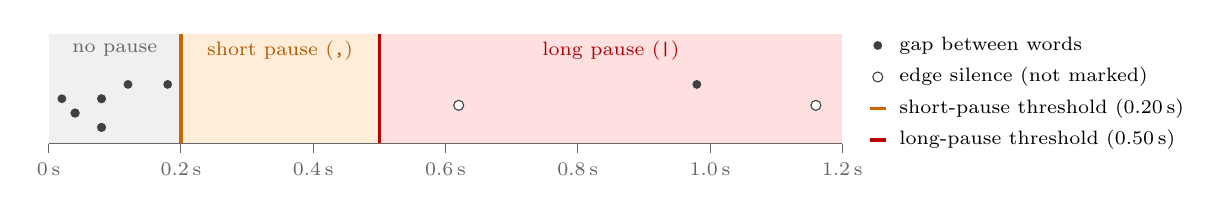
\begin{tikzpicture}[x=8.4cm, y=1.4cm,
    legend/.style={font=\scriptsize, anchor=west},
  ]
  \def\axisend{1.2}

  % Regions: no pause, short pause and long pause
  \fill[black!6]   (0,0)               rectangle (\shortthreshold,1);
  \fill[orange!15] (\shortthreshold,0) rectangle (\longthreshold,1);
  \fill[red!12]    (\longthreshold,0)  rectangle (\axisend,1);

  % Silences, stacked in four rows so that equal values do not hide each other
  \foreach [count=\i] \gap in \innergaps
    \fill[black!75] (\gap,{0.15 + mod(\i,4)*0.13}) circle (1.6pt);
  \foreach \gap in \edgegaps
    \draw[black!75, fill=white] (\gap,0.35) circle (1.8pt);

  % The two thresholds
  \draw[orange!80!black, line width=1.2pt] (\shortthreshold,0) -- (\shortthreshold,1);
  \draw[red!75!black,    line width=1.2pt] (\longthreshold,0)  -- (\longthreshold,1);

  % Region labels
  \node[font=\scriptsize, text=black!60, fill=black!6, inner sep=1pt]
    at ({\shortthreshold/2},0.85) {no pause};
  \node[font=\scriptsize, text=orange!70!black, fill=orange!15, inner sep=1pt]
    at ({(\shortthreshold+\longthreshold)/2},0.85) {short pause (\texttt{,})};
  \node[font=\scriptsize, text=red!70!black, fill=red!12, inner sep=1pt]
    at ({(\longthreshold+\axisend)/2},0.85) {long pause (\texttt{|})};

  % Axis
  \draw[black!60] (0,0) -- (\axisend,0);
  \foreach \t in {0,0.2,0.4,0.6,0.8,1.0,1.2}
    \draw[black!60] (\t,0) -- ++(0,-0.08) node[below, font=\scriptsize] {\t\,s};

  % Legend, beside the diagram (positions in cm)
  \begin{scope}[shift={(\axisend,0)}, x=1cm, y=1cm, xshift=0.35cm]
    \fill[black!75] (0.1,1.25) circle (1.6pt);
    \node[legend] at (0.25,1.25) {gap between words};
    \draw[black!75, fill=white] (0.1,0.85) circle (1.8pt);
    \node[legend] at (0.25,0.85) {edge silence (not marked)};
    \draw[orange!80!black, line width=1.2pt] (0,0.45) -- (0.2,0.45);
    \node[legend] at (0.25,0.45) {short-pause threshold (\shortthreshold\,s)};
    \draw[red!75!black, line width=1.2pt] (0,0.05) -- (0.2,0.05);
    \node[legend] at (0.25,0.05) {long-pause threshold (\longthreshold\,s)};
  \end{scope}
\end{tikzpicture}

\end{center}

Only the pause marker is written into the transcribed sentence:

\smallskip
\begin{center}{\bn গ্রেগরির কাছ থেকে এখনও উত্তর পেলাম না {\color{red!75!black}\textbf{|}} সে কি তাহলে ইংল্যাণ্ডে নেই}\end{center}
\end{example}

%=====================================================================
\section{Translation}
%=====================================================================

Translation is performed by the translation model (Table~\ref{tab:models}). The model receives a one-line instruction, \emph{``Translate the following text into English''}, followed by the Bengali text. The translation is generated greedily, without sampling, so the same input always gives the same output.

Two versions of the sentence are translated:
\begin{itemize}[nosep]
  \item The \textbf{clean} sentence is the transcript without any markers.
  \item The \textbf{marked} sentence contains the pause markers from the alignment and prosody marking stage.
\end{itemize}
Comparing the two versions shows the effect of the markers on the translation of the example. The marked translation is used for synthesis.

\begin{example}[: translation]
The diagram aligns the marked Bengali with both English translations, and the punctuation and capital letters that the translator added are highlighted. \textbf{Without the marker, the question was no longer marked as a question.} For this clip, the output with the marker is consistent with the intended effect of the pause markers.

\begin{center}
% Worked example, Stage 4: the marked Bengali, split at its long-pause bar, mapped to the
% two sentences of the marked English translation, with the unmarked translation below.
% Punctuation and capital letters that the translator added are shown in red.
\begin{tikzpicture}[
    bengali/.style={draw=blue!55!black, fill=blue!5, rounded corners=3pt, align=center,
                    anchor=north, inner sep=5pt},
    english/.style={draw=green!40!black, fill=green!5, rounded corners=3pt, align=center,
                    anchor=north, inner sep=5pt, font=\small,
                    execute at begin node={\hyphenpenalty 10000\relax}},
    bar/.style={text=red!75!black, font=\Large\bfseries},
    row title/.style={font=\footnotesize\bfseries, anchor=south west},
    maps to/.style={-{Stealth[length=2mm]}, black!60, line width=0.8pt},
    note/.style={font=\scriptsize\itshape, text=violet, align=center},
  ]
  % added punctuation and capitals: bold red letters
  \def\hl#1{\textbf{\color{red!80!black}#1}}

  % Marked Bengali: two phrases separated by one long-pause bar
  \node[row title] at (0.3,0.1) {Marked Bengali};
  \node[bengali, text width=7.4cm] (b1) at (4.2,0) {\bn গ্রেগরির কাছ থেকে এখনও উত্তর পেলাম না};
  \node[bar] at (8.35,0 |- b1.center) {|};
  \node[bengali, text width=5.2cm] (b2) at (11.45,0) {\bn সে কি তাহলে ইংল্যাণ্ডে নেই};

  % Marked English: the bar became a sentence break and was not copied
  \coordinate (row2) at ([yshift=-14mm]b1.south);
  \node[english, text width=7.4cm] (e1) at (4.2,0 |- row2)
    {\hl{I} haven't received a reply from \hl{G}regory yet\hl{.}};
  \node[english, text width=5.2cm] (e2) at (11.45,0 |- row2)
    {\hl{I}s he not in \hl{E}ngland\hl{?}};
  \node[row title] at ([yshift=1mm]0.3,0 |- e1.north) {Marked English};
  \node[note] at ($(8.35,0 |- b1.south)!0.5!(8.35,0 |- e1.north)$)
    {the bar was not copied;\\a sentence break appeared};
  \draw[maps to] (b1.south) -- ([yshift=1mm]e1.north);
  \draw[maps to] (b2.south) -- ([yshift=1mm]e2.north);

  % The same sentence translated without markers
  \node[row title, anchor=north west] (clean) at ([yshift=-5mm]0,0 |- e1.south) {English without markers};
  \node[draw=black!50, fill=black!4, rounded corners=3pt, text width=13.6cm, align=center,
        anchor=north west, inner sep=5pt, font=\small] (c) at ([xshift=0.3cm]clean.south west)
    {i haven't received a reply from gregory yet is he not in england};
  \node[note, text=black!60, anchor=north] at (c.south) {one run-on string: no punctuation and no capital letters};
\end{tikzpicture}

\end{center}
\end{example}

%=====================================================================
\section{Voice-Cloned Speech Synthesis}
%=====================================================================

The English translation is spoken by the speech synthesis model (Table~\ref{tab:models}), which can clone a voice from a short reference recording without any training.

The model receives three inputs:
\begin{itemize}[nosep]
  \item The first input is the English text to be spoken, which is the marked translation.
  \item The second input is the original Bengali clip, which serves as the voice reference.
  \item The third input is a transcript of that reference. The pause-marked Bengali is used here, so that the transcript matches the reference audio as closely as possible.
\end{itemize}
Generation uses sampling with a temperature of 0.8 and top-50 sampling. The output is English speech at \textbf{24\,kHz} in the original speaker's voice.

\begin{example}[: speech synthesis]
The diagram shows the three inputs that the speech synthesis model received and the speech it produced.

\begin{center}
% Worked example, Stage 5: the inputs to the speech synthesis model and the speech it produced.
\begin{tikzpicture}[
    input/.style={draw=black!55, fill=black!4, rounded corners=3pt, text width=5.9cm,
                  align=left, inner sep=5pt, font=\small,
                  execute at begin node={\hyphenpenalty 10000\relax}},
    stage/.style={rounded corners=4pt, line width=0.8pt, align=center, inner sep=6pt,
                  execute at begin node={\hyphenpenalty 10000\relax}},
    flow/.style={-{Stealth[length=2.2mm]}, black!60, line width=0.8pt},
  ]
  \def\bigicon{\fontsize{20}{20}\selectfont}

  % Inputs, model and output
  \node[input] (text)  at (3.1,0)    {\faIcon{file-alt}\ \textbf{Text to speak}\\[2pt] \footnotesize I haven't received a reply from Gregory yet. Is he not in England?};
  \node[input] (voice) [below=3mm of text] {\faIcon{microphone}\ \textbf{Voice reference}\\[2pt] \footnotesize the original Bengali clip};
  \node[input] (ref)   [below=3mm of voice] {\faIcon{file-alt}\ \textbf{Reference transcript}\\[2pt] {\bn গ্রেগরির কাছ থেকে এখনও উত্তর পেলাম না {\color{red!75!black}\textbf{|}} সে কি তাহলে ইংল্যাণ্ডে নেই}};
  \node[stage, draw=blue!55!black, fill=blue!7, text width=3.2cm] (model) at (8.85,0 |- voice)
    {{\color{blue!55!black}\bigicon\faIcon{volume-up}}\\[3pt]
     \small\textbf{Speech synthesis model}\\ \footnotesize zero-shot cloning};
  \node[stage, draw=green!40!black, fill=green!6, text width=2.9cm] (out) at (12.95,0 |- voice)
    {{\color{green!40!black}\bigicon\faIcon{headphones}}\\[3pt]
     \small\textbf{English speech}\\ \footnotesize in the original voice};
  \foreach \n in {text, voice, ref}
    \draw[flow] (\n.east) -- (model.west);
  \draw[flow] (model.east) -- (out.west);
\end{tikzpicture}

\end{center}
\end{example}

%=====================================================================
\section{Observations and Open Issues}
%=====================================================================

\begin{itemize}
  \item \textbf{Loudness and elongation are not yet used.} They are measured but are not passed to the translator or the synthesizer. Whether these models can make use of such markers remains an open question.
  \item \textbf{Foreign names are romanized poorly.} Names from other languages that are written in Bengali script are romanized letter by letter, so their Latin spelling does not match their pronunciation. In the worked example, {\bn গ্রেগরির} became \texttt{gregarir} and {\bn ইংল্যাণ্ডে} became \texttt{inglyaanndde}, and the doubled letters in the latter made its elongation measure understate how long it lasted.
\end{itemize}


\printbibliography

\end{document}
